\documentclass[conference]{IEEEtran}

% The following packages can be found on http:\\www.ctan.org
\usepackage[utf8]{inputenc}
\usepackage{graphicx}
\usepackage{makeidx}
\usepackage[caption=false]{subfig}
%\usepackage{subfigure}
%\usepackage{subcaption}
\usepackage{lscape}
\usepackage{float}
\usepackage{hyperref}
\IEEEoverridecommandlockouts  % This command is only needed if 
                              % you want to use the \thanks command
\overrideIEEEmargins          % Needed to meet printer requirements.

% See the \addtolength command later in the file to balance the column lengths
% on the last page of the document

\title{\LARGE \bf
RoboIME: on the road to LARC 2014
}


%\author{Albert Author$^{1}$ and Bernard D. Researcher$^{2}$% <-this % stops a space
%\thanks{*This work was not supported by any organization}% <-this % stops a space
%\thanks{$^{1}$Albert Author is with Faculty of Electrical Engineering, Mathematics and Computer Science,
%        University of Twente, 7500 AE Enschede, The Netherlands
%        {\tt\small albert.author@papercept.net}}%
%\thanks{$^{2}$Bernard D. Researcheris with the Department of Electrical Engineering, Wright State University,
%        Dayton, OH 45435, USA
%        {\tt\small b.d.researcher@ieee.org}}%
%}

\author{
  \IEEEauthorblockN{%
    Driele N. Ribeiro \and
    Gabrielle B. do Nascimento \and
    Jan L. L. Segre \and
    Lucas O. de Lima \and
    Naum A. F. Barreira \and
    Marina M. de Lima \and
    Rafhael J. Lima \and
    Renan Gemignani \and
    Robinson Calou M. B. Filho \and
    Vitor H. F. Bettio \and
    Victor L. H. Ferreira \and
    Victor Bramigk \and
    Paulo F. F. Rosa}%
  \IEEEauthorblockA{%
    Instituto Militar de Engenharia,
    %Praça General Tibúrcio, 80 - Praia Vermelha, Urca,
    Praca General Tiburcio, 80 - Praia Vermelha, Urca,
    Rio de Janeiro RJ, Brasil}%
    %{\tt\small roboime@googlegroups.com}}%
}

%\author{\IEEEauthorblockN{Michael Shell\IEEEauthorrefmark{1},
%Homer Simpson\IEEEauthorrefmark{2},
%James Kirk\IEEEauthorrefmark{3}, 
%Montgomery Scott\IEEEauthorrefmark{3} and
%Eldon Tyrell\IEEEauthorrefmark{4}}
%\IEEEauthorblockA{\IEEEauthorrefmark{1}School of Electrical and Computer Engineering\\
%Georgia Institute of Technology,
%Atlanta, Georgia 30332--0250\\ Email: see http://www.michaelshell.org/contact.html}
%\IEEEauthorblockA{\IEEEauthorrefmark{2}Twentieth Century Fox, Springfield, USA\\
%Email: homer@thesimpsons.com}
%\IEEEauthorblockA{\IEEEauthorrefmark{3}Starfleet Academy, San Francisco, California 96678-2391\\
%Telephone: (800) 555--1212, Fax: (888) 555--1212}
%\IEEEauthorblockA{\IEEEauthorrefmark{4}Tyrell Inc., 123 Replicant Street, Los Angeles, California 90210--4321}}

\graphicspath{{img/}}


\begin{document}

\maketitle

\begin{abstract}
This paper describes the electronic, mechanical and software designs developed by RoboIME
Team in order to join RoboCup \the\year. All designs are in agreement with the rules of Small
Size League \the\year. This is the third RoboIME participation in a world level RoboCup event,
% TODO: Correct number of challenges
although the team has already been challenged three times in competitions in Brazil and Latin America.
\end{abstract}

\section{Introduction}
RoboIME is a small-size league soccer robot team from IME, Rio de Janeiro, Brazil. This
is only the 5th time the team is taking part in competitions. The biggest result achieved was in 2012
when the team achieved second place in Latin American Robotics Competition.

All students that work in this project are members of the Laboratório de Robótica e
Inteligência Computacional at IME. Previous studies \cite{alexandre}\cite{marco} provided
the basis for the current structure of software and hardware teams. This paper describes the
computer, electronic and mechanical designs.

This work is organized as follows. The mechanical design of RoboIME robots is presented in section \ref{mec_sec}. Then the firmware and electrical project is presented in section \ref{emb_sys_sec}. The software system is presented in section \ref{soft_sys_sec}. Finally, discussion and future work are described in section \ref{dic_fut_sec}.

%\section{Literature Review}

TODO: Talk about references \cite{tdp}, \cite{STP} and \cite{zickler}.

\section{Embedded System}\label{emb_sys_sec}
RoboIME electronics consist of nine boards: (a) the Main board, responsible for communication between the other boards; (b) the Stamp board, responsible for the embedded computations; (c) the Kicker board, responsible for maintaining high voltage and activate the kickers; (d) five motor controller boards which are responsible for the robot's motion control and the dribbling device. (e)Transceiver board, which is responsible for the link between the robot and the main computer. These boards are described in details in this section.

\subsection{Main Board}
The Main Board features a socket to plug the boards in: the kicker's sensor, a optical sensor that is used to detect if the robot is with the ball possession, dribbler motor, which makes possible to the robot to spin and to move backward without lose the ball, four wheels' motors, four quadrature encoders and the power supply with safety devices.

\subsection{Stamp Board}
This board is responsible  for performing all the logical functions. Serving as a brain of sorts for the electronic system. There is an embedded STM32F407VG micro-controller, with an ARM Cortex M4 as main CPU, 1 MB Flash, 192 KB RAM memory, working at 168 MHz, that was programmed in C language using CoIDE and Eclipse IDEs. The main function of the embedded system is to receive the data from the AI and convert it into movement. So, there is a Proportional Derivative Integrative Control sampling the real wheel's velocity, comparing with the desired and outputting the appropriate voltage to the motor. That control has the fundamental importance of look for the right wheel's velocity. There is also a current control that doesn't permit the Motor Controller Board to burn out.
%vide http://www.st.com/st-web-ui/static/active/en/resource/sales_and_marketing/promotional_material/brochure/brstm32f4.pdf

\subsection{Kicker Board}
This board is responsible for produce the high voltage used to activate the two coils, controlling the kick strength and discharge almost instantly all the power stored on the coils. There are two kinds of kick, the forward kick and the high kick. There are two steps in this board: charge and discharge. The first has the unique function of keep a constant output of 180V DC from a input of 7~8V DC. A DC-DC step-up power supply controlled by the MC34063 IC and two electrolytic capacitors of 2200 $\mu$F, 200 V are used for this task. The second is to drive the kickers. In this part are used one TC4427 Mosfet Driver IC and two IRFP4868PBF Power Mosfet that are responsible for close the high voltage circuit of the first step with the ground through the coil, converting electrical into mechanical energy. A precise control of the actuation time ensure that the kick will occur with the right velocity.

%include image of high kick

\subsection{Motor Controller Board}
The idea of the RoboIME electronic is to modularize the electronic project. So, there is one controller module board for each wheel motor. If one of them burns out, it is possible to exchange it quickly. Each board has two TC4427 (MOSFET driver) and two IRF7319 (complementary half H bridge). These ICs create an H-bridge, allowing the velocity control in both directions through a Pulse-Width Modulation, converting a digital signal input into an analog output.


\subsection{Transceiver Board}
The transceiver board is responsible for the link between the micro-controller and the main computer through a RFM12B transceiver. The first is done using a own protocol, operating in the 434 MHz band, simplex, set up for 20 kbps, fully compliant with FCC and ETSI regulations. The second is accomplished through the Serial Peripheral Interface Bus (SPI), a standard

\section{Mechanical Design}\label{mec_sec}

This robot was designed and built using CAD (Computer Aided Design) and CAM
(Computer Aided Manufacturing) software. Moreover, extensive testing was done
to validate the current project.

Most of our robot parts were CNC machined and made out of 7075 aluminium and
high density polyoxymethylene (POM). The POM have some excellent prop- erties
such as high rigidity, good impact resistance, a non-stick characteristic and
beng a highly machinable material. In this way, some parts of the robots, like
the plunger stopping body, are more suitable to be made out of POM than
aluminium. For example, the dribbler arm is a pivot-rotating mechanism, and
using POM eliminates the need for a bearing within the assembly.

%\begin{figure}[thpb]
%    \centering
%    \begin{subfigure}[b]{0.49 \textwidth}
%        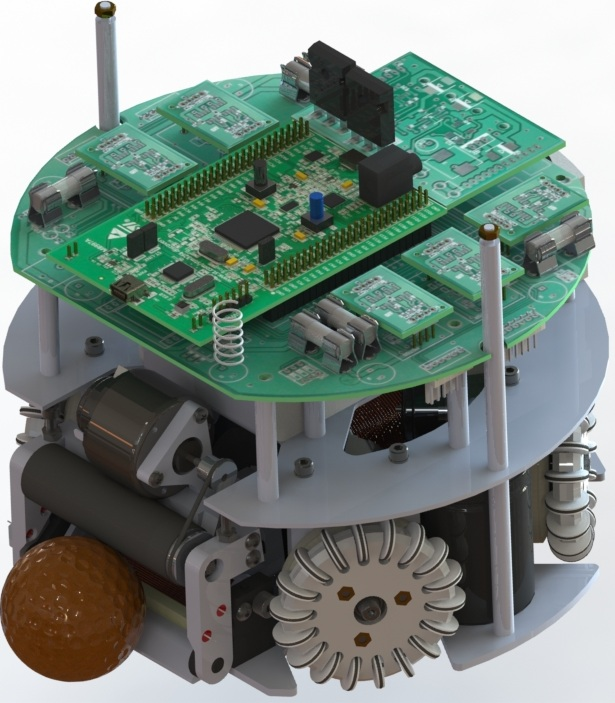
\includegraphics[width=\linewidth]{modeladof2}
%        \caption{3D model view.}
%        \label{fig:modelado}
%    \end{subfigure}
%    \begin{subfigure}[b]{0.49 \linewidth}
%        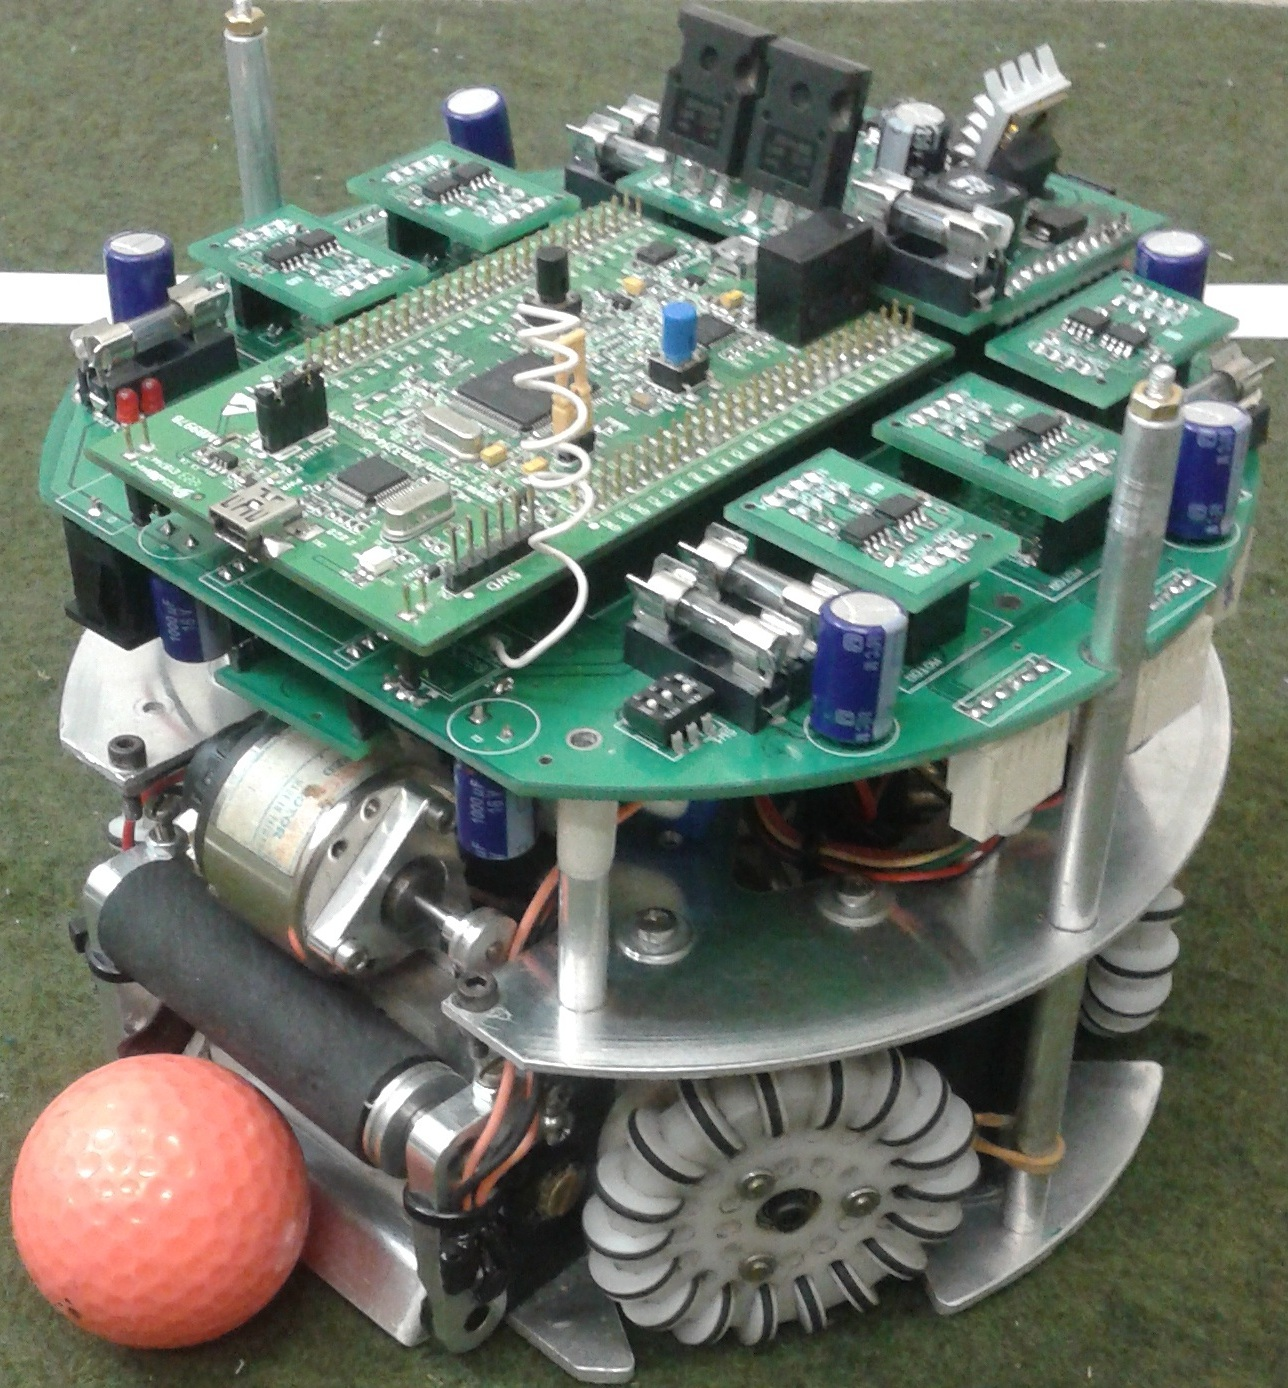
\includegraphics[width=\linewidth]{realf2}
%        \caption{Real robot view.}
%        \label{fig:real}
%    }
%    \end{subfigure}
%\end{figure}

\begin{figure}[ht]
    \subfloat[]{%
        \label{fig:modelado}
        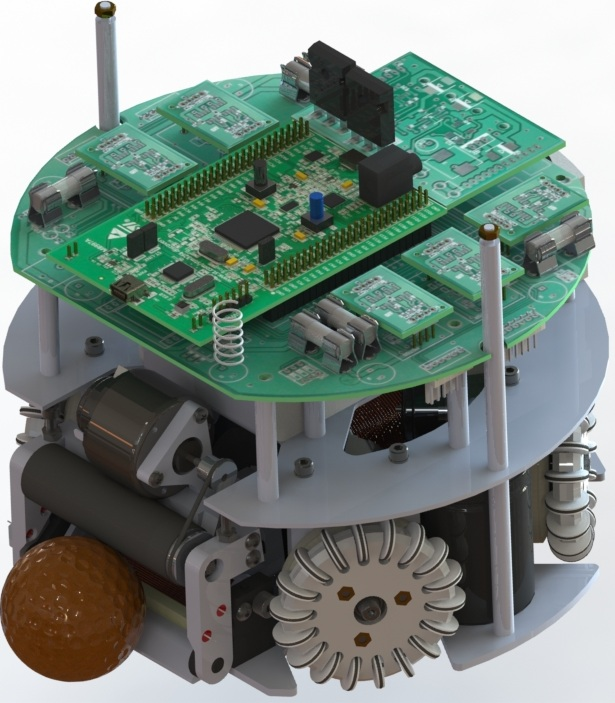
\includegraphics[width=0.47\linewidth]{modeladof2}
    }
    \subfloat[]{%
        \label{fig:real}
        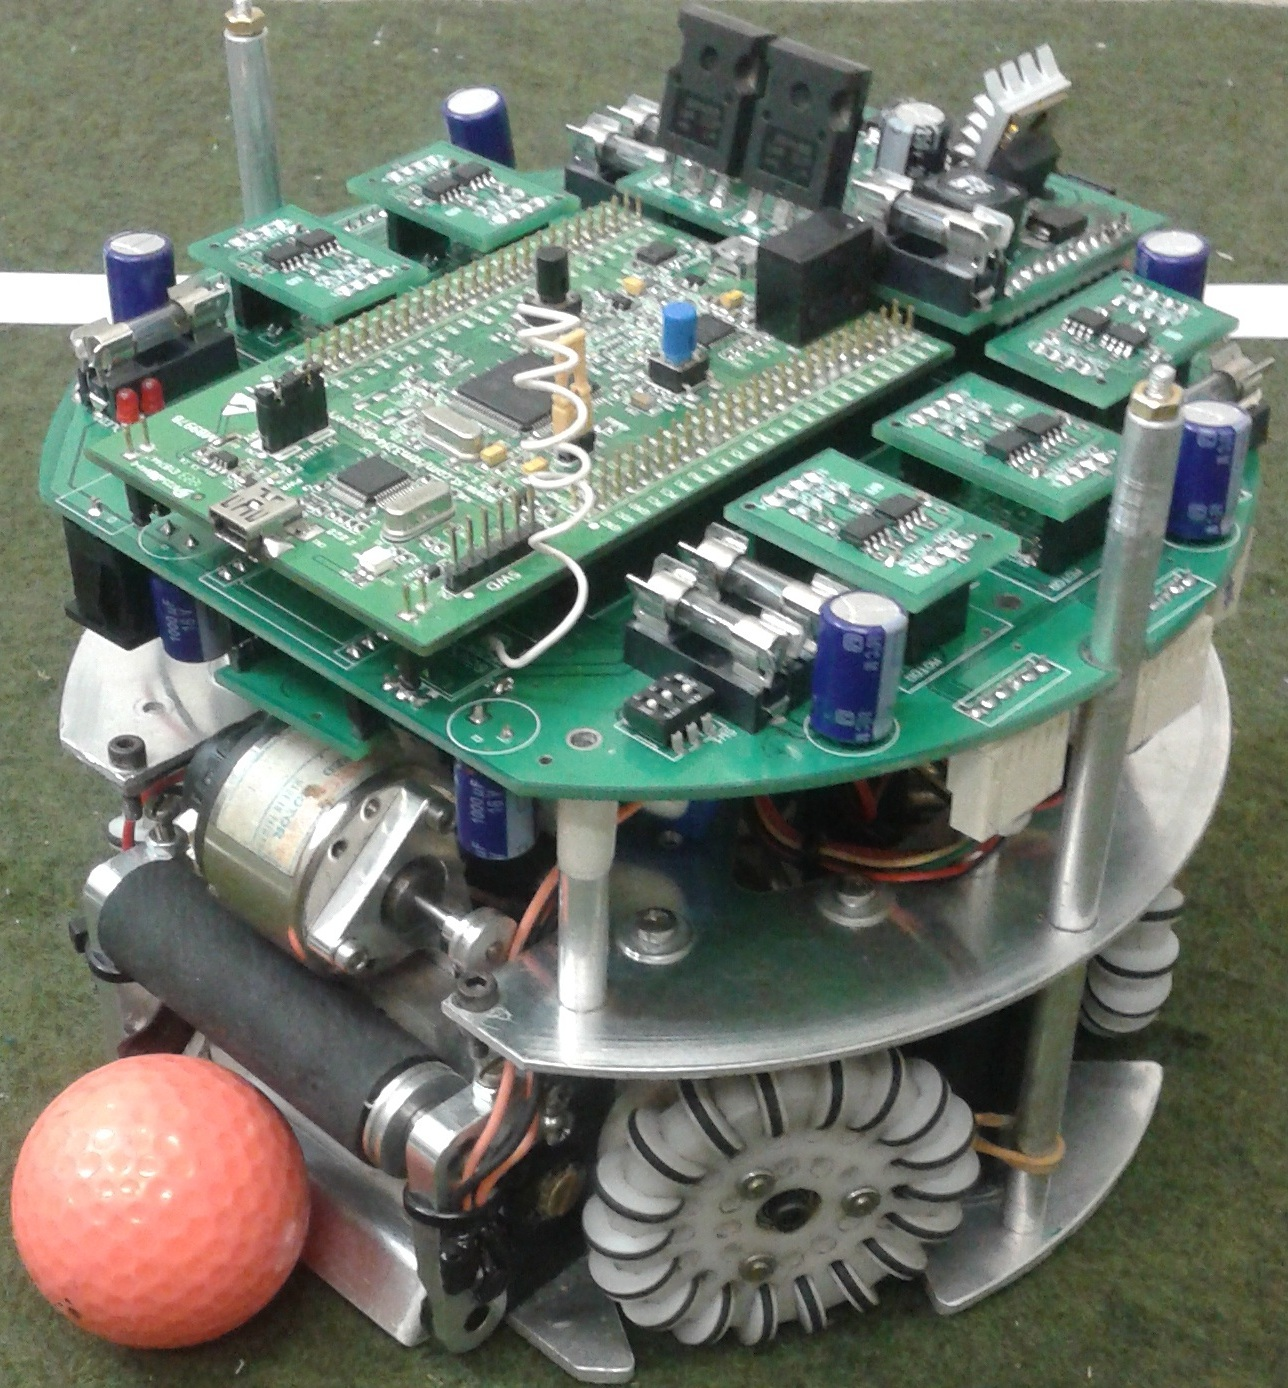
\includegraphics[width=0.47\linewidth]{realf2}
    }
    \label{fig:real_and_model}
    \caption{3D model~\ref{fig:modelado} and real robot~\ref{fig:real} views.}
\end{figure}


\subsection{Dimensional Constraints}
In compliance with the SSL rules, the height of the robot is 149 mm and the
maximum projection of the robot on the ground is 180 mm.

\begin{figure}[ht]
    \centering
    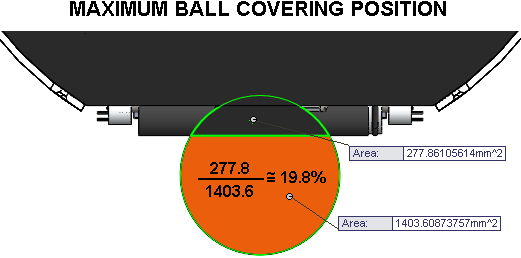
\includegraphics[width=\linewidth]{20-80_rule}
    \caption{Maximun covered area of the ball.}
    \label{fig:20-80_rule}
\end{figure}

Using CAD software we were able to measure the percentage of the ball area that
was covered by the robot. The maximum percentage of ball coverage found was
19,8\%, in accordance to the 20/80 rule of the league. The height of the
dribbler cylinder is also adjustable, so we are able to find the optimum point
for the best ball control.


\subsection{Transmission System}

A system of internal gears was made to transfer the power of the motors to the
wheels. This system has several advantages compared to traditional gear
meshing, such as avoiding debris entering the motors, creating a cavity to
apply grease for lubrication of gears and an overall smaller size.

However there are some difficulties in the manufacturing of this part, mainly
due to the small size of the teeth needed to mesh with standard motor gear (the
motor being used is the Hsiang Neng DC brushed motor type HN-GH35GMB). At this
motor the distance between two consecutive teeth is less than 1 mm, thus it was
not feasible to machine the internal gear. So it was decided for 3D printing in
ABS plastic as the manufacturing process.

The traditional fused filament deposition method for 3D printing, in geometries
smaller than the filament itself, create cavernous structures that weaken the
piece. Applying the stereolithography 3D printing process (when a laser beam
cure a liquid resin layer by layer), we manage to achieve a higher resolution.
This way we can precisely print the teeth profile, avoiding failures due to
empty spots and achieving a more solid and precise component.


\subsection{Chip Kick}

The chip kick is based on a flat solenoid, which is mounted in a slot at the
chassis (close to the ground). When activated the core of mild steel is
accelerated against the rear of the chip, which revolves around its axis and
makes the ball rise. Due to the limited space, complex construction and
details, we also have chosen the 3D printing as the manufacturing process.


\begin{figure}[tbph]
    \centering
    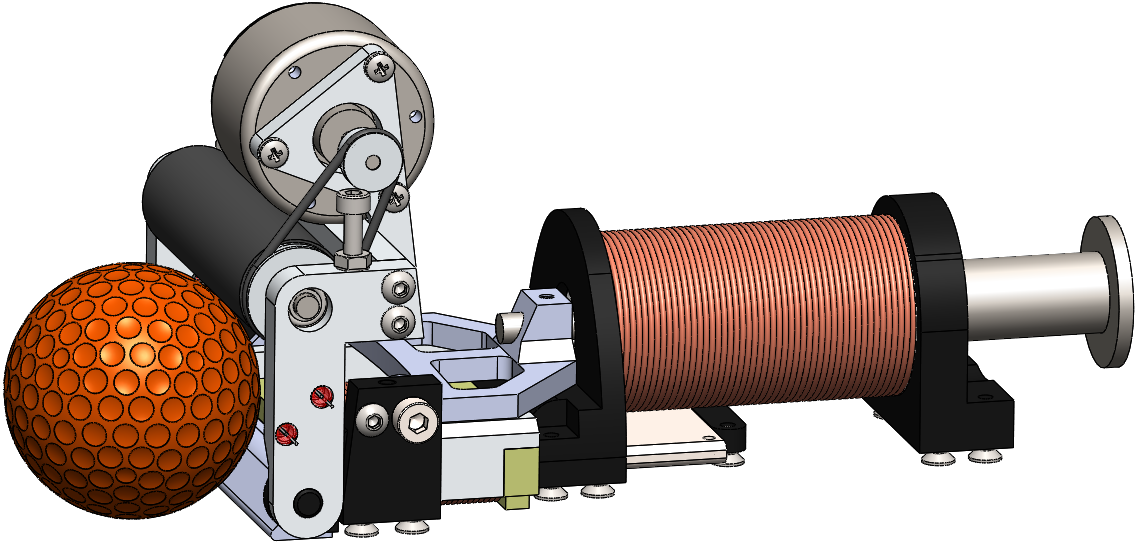
\includegraphics[width=\linewidth]{fechado}
    \caption{Dribbler, chipper and kicker assembly.}
    \label{fig:fechado}

    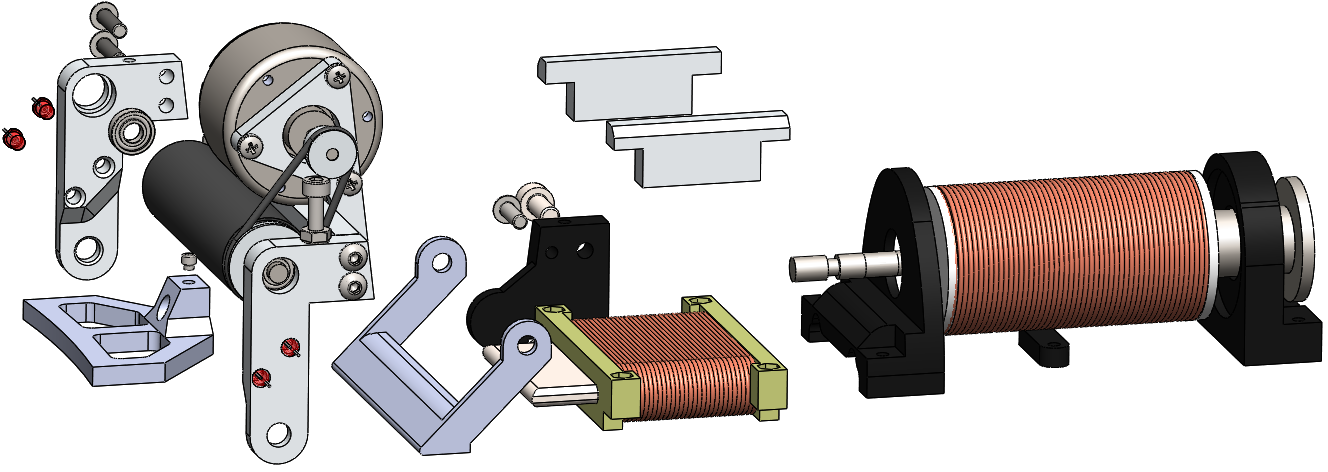
\includegraphics[width=\linewidth]{explodida}
    \caption{Exploded view.}
    \label{fig:explodida}
\end{figure}

The flat solenoid is assembled in a way that works as a guide rail for the kick
plunger as well. We are using rubber bands to pull back the chipper and kicker
plungers, keeping the mechanism simple. The final dribbling/kicking mechanism
is a very neat assembly and can be easily adapted for any other chassis.

% vim: tw=79 et sw=4 ts=4 filetype=tex

\section{Software Solutions}\label{soft_sys_sec}

The software systems consist of three projects: pyroboime (AI), ssl-webclient (graphical client), grSim (simulator).

\subsection{Artificial Intelligence}

The AI, pyroboime, is based on the STP (Skill-Tactic-Play) architecture and implemented in python.
It has the following components: interface with the ssl-vision, ssl-refbox and grSim, it also has a built-in communication module for the radio transmitter system.
%The block diagram of the AI software is presented in figure \ref{fluxogramSoftware}.

The STP is a three tier architecture where the lowest level, skills, enables the low level manipulations on a single robot.
The middle layer, tactics, makes use of the skill layer to execute higher level behaviour, possibly enabling coopration, but still acting on a single robot.
The upper layer, plays, coordinates the tactics associated to each robot in order to maximize performance, each play is implemented to behave according to specific states: stop, halt, indirect kicks and normal play.
A higher level layer implmented as a play switches between other plays based on the current referee state.
This architecture is better depicted in figure \ref{STPDiagram}.

\begin{figure}[H]
     \centering
     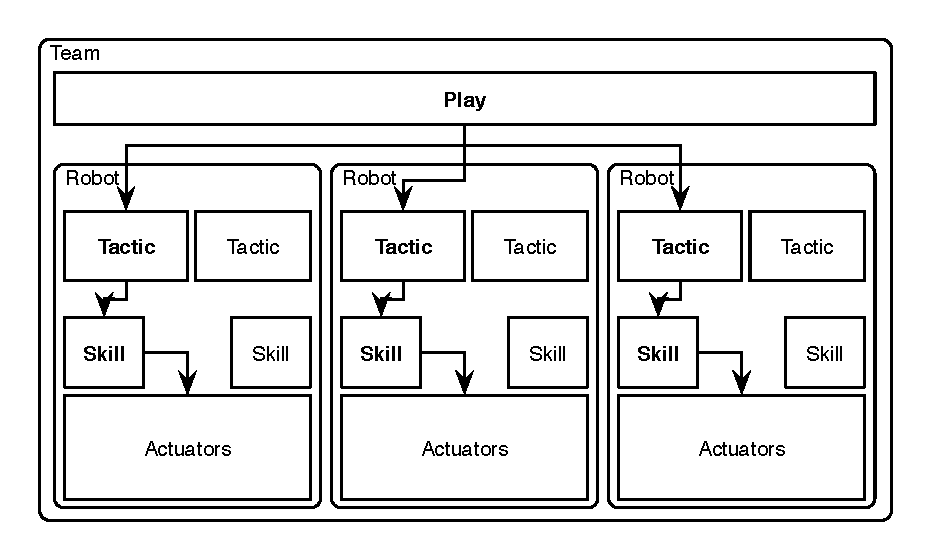
\includegraphics[width = \linewidth]{stp}
     \caption{STP Diagram}
     \label{STPDiagram}
\end{figure}

There is also a skill implemented to redirect inputs from a joystick such that it is possible to test the robot with little effort.

The interface is structured as a filter stack which connects the AI to a flexible collection of updaters (which receive state information) and commanders (which deliver commands to the robots, in both the simulated and real environments).
It abstracts the external environment where the game is played from the AI.
Among the filters in said stack is a Kalman filter that reduces the noise comming from the updater data.

The built-in radio trasmitter system interfaces with libusb to control the transmitter hardware, which is connected via USB.

%\begin{landscape}
%\begin{figure}[H]
%     \centering
%     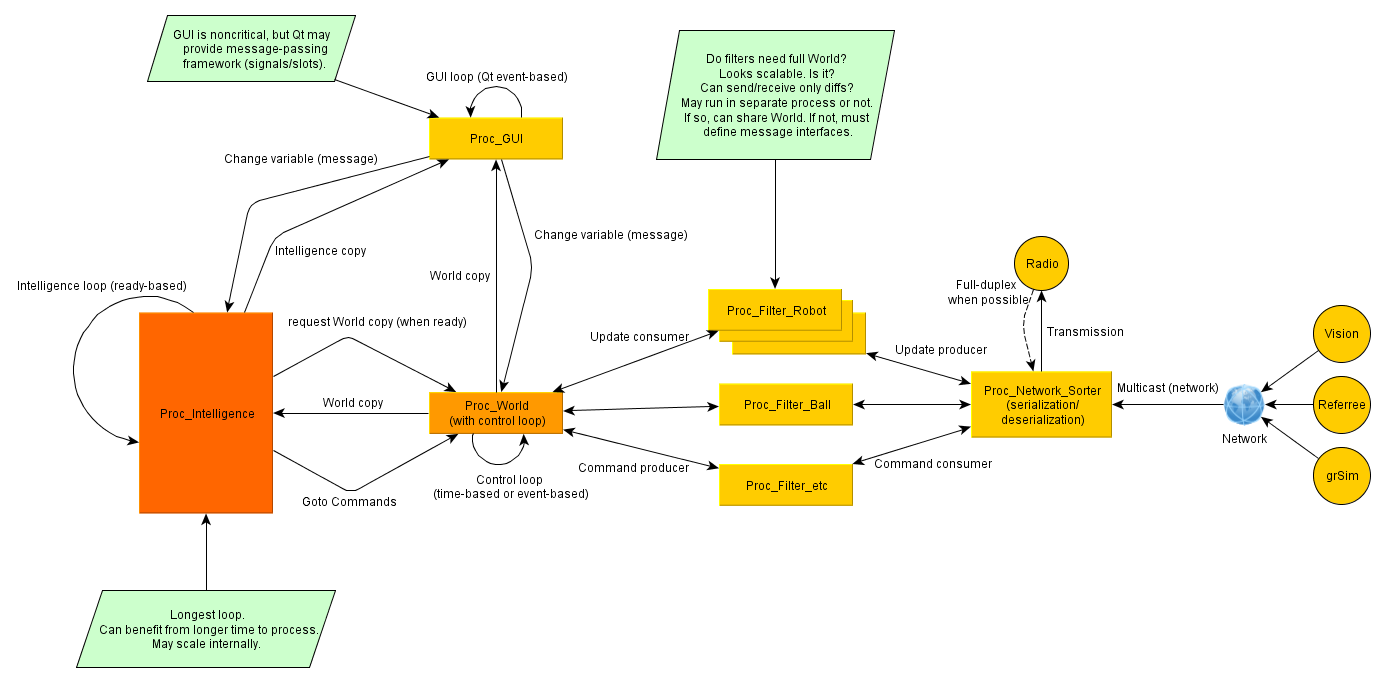
\includegraphics[width = \linewidth]{software-model}
%     \caption{Block diagram of the AI software}
%     \label{fluxogramSoftware}
%\end{figure}
%\end{landscape}

\subsection{Support systems}

The graphical client, ssl-webclient, is a Web interface implemented in nodejs using WebSockets, HTML5, SVG and ZeroMQ.
It has the following functionality: displaying and altering the AI state, broadcasting games through the internet and playing log files.

Lastly the simulator, grSim, originally developed by Parsian Robotic, was customized to fit our needs.
It provides the following functionality: simulating the game environment and exposing an ssl-vision compliant protocol.

\begin{figure}[H]
     \centering
     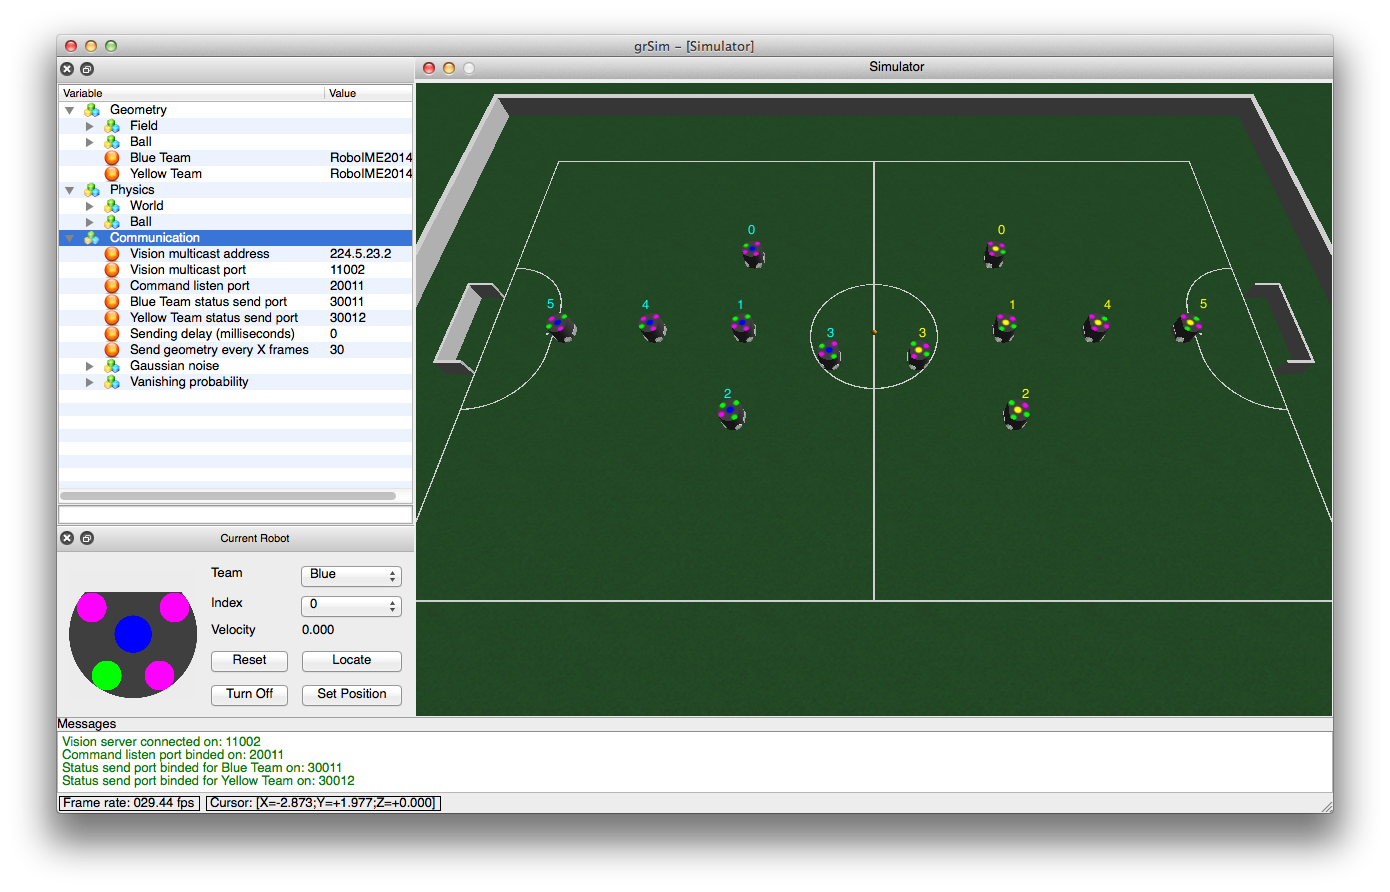
\includegraphics[width = \linewidth]{grsim}
     \caption{Snapshot of the simulator}
     \label{simulatorSnapshot}
\end{figure}

\subsection{Source}

All of the projects above have been open sourced with GPL-like license, with the main difference being that a derived work used on a competition must have its source released by the next edition of that competition. The sources of those projects are available on the team's github page: \url{http://github.com/roboime/}.

\section{Discussion and Future Works}\label{dic_fut_sec}

The development of the mechanical project was concluded last year, based on the
one we created for Brazilian Robotics Competition 2012. The six robots have
already been manufactured, with only a few parts still needing rework.

Some electronic prototypes were made, yet stabilizing efforts are still
ongoing. Problems with kicker board due to hight welding temperature were
observed. The solution was to use a welding temperature below
$260\,^{\circ}\mathrm{C}$.

The five modules of the AI system have already been implemented but they still
need to be brought to perfection. Research in machine learning was started last
year to predict enemy behaviour, but an implementation is not planned for this
competition.

For the this competition, following goals are being sought: rework the
remaining parts on the mechanical project such as making improvements on the
coiling of the solenoid coil; stabilize the electronic project, including robot
feedback and conclude the implementation of planning algorithms to be used in
support decision making.

% vim: tw=79 et sw=4 ts=4 filetype=tex


% This command serves to balance the column lengths
% on the last page of the document manually. It shortens
% the textheight of the last page by a suitable amount.
% This command does not take effect until the next page
% so it should come on the page before the last. Make
% sure that you do not shorten the textheight too much.
\addtolength{\textheight}{-12cm}

\section*{Acknowledgements}

This research was partially supported by Funda\c c\={a}o Carlos Chagas Filho de
Amparo \`{a} Pesquisa do Estado do Rio de Janeiro - FAPERJ(grant
E-26/111.362/2012); Funda\c c\={a}o Ricardo Franco (FRF) and F\'{a}brica de
Material de Comunica\c c\={a}o e Eletr\^{o}nica (FMCE/IMBEL). The team also
acknowledges the assistance of Mr. Carlos Beckhauser from FMCE\@. Special thanks
to Diego Felix de Almeida, Luis Renault L. Rodrigues, Stefano H. Rodrigues,
Thiago A. Navarro do Amaral and Victor L. Horta Ferreira, former team members
that made this project possible.

% vim: tw=79 et sw=4 ts=4 filetype=tex

\begin{thebibliography}{7}
%%%%%%%%%%%%%%%%%%%%%%

\bibitem{alexandre}
Alexandre Tadeu Rossini da Silva:
Comportamento social cooperativo na realização de tarefas em
ambientes dinâmicos e competitivos.
Instituto Militar de Engenharia, Rio de Janeiro (2006)

\bibitem{tdp}
Madeira, B.~E., de~Almeida, D.~F., de~C.~Maia~Jr., E., Rodrigues, L. R.~L.,
  Rosa, P. F.~F., Rodrigues, S.~H., and do~Amaral, T. A.~N.:
RoboIME: Team Description Paper for RoboCup 2012.

\bibitem{STP}
B. Browning and J. Bruce and M. Bowling and M. Veloso:
STP: Skills, tactics and plays for multi-robot control in adversarial environments
Carnegie Mellon University, Pittsburgh, PA (2004)

\bibitem{CPA}
Khatib, O.:
Real-Time Obstacle Avoidance for Manipulators and Mobile Robots.
In International Journal of Robotics Research, vol. 5, no. 1, p. 90-98 (1986)

\bibitem{marco}
Marco Antonio Firmino de Sousa:
Uma Plataforma para Cooperação Autónoma de Múltiplos Robôs
Instituto Militar de Engenharia, Rio de Janeiro (2008)

\bibitem{minimax} Russell, Stuart J.; Norvig, Peter:
Artificial Intelligence: A Modern Approach (2nd ed.)
Upper Saddle River, New Jersey: Prentice Hall, pp. 163-171 (2003)

\bibitem{zickler}
Stefan Zickler:
Physics-Based Robot Motion Planning in Dynamic Multi-Body Environments
Carnegie Mellon University, Pittsburgh, PA (2010)

\bibitem{ekf}
Welch, G. and Bishop, G.:
An introduction to the Kalman filter. Technical Report TR 95-041, Department of
Computer Science, University of North Carolina (2001)


%\bibitem{simCamera}
%Stefan Zickler, Olivier Michel:
%SSL-vision Webots integration
%http://youtu.be/sRAVELC8jKM, 26/02/2012


\end{thebibliography}


\end{document}

% vim: et sw=2 ts=2 tw=79
